\documentclass{beamer}
%
% Choose how your presentation looks.
%
% For more themes, color themes and font themes, see:
% http://deic.uab.es/~iblanes/beamer_gallery/index_by_theme.html
%
\mode<presentation>
{
  \usetheme{default}      % or try Darmstadt, Madrid, Warsaw, ...
  \usecolortheme{default} % or try albatross, beaver, crane, ...
  \usefonttheme{default}  % or try serif, structurebold, ...
  \setbeamertemplate{navigation symbols}{}
  \setbeamertemplate{caption}[numbered]
} 

\usepackage[english]{babel}
\usepackage[utf8x]{inputenc}
\usepackage{multirow}
\usepackage{booktabs}
\usepackage{bigstrut}
\usepackage{hyperref}


\begin{document}




\begin{frame}{Datasets}

\begin{table}[]
    \centering
    \begin{tabular}{cccc}
    \toprule  
    Datasets & Users & Items & Ratings\\
    \midrule  
    Instant Video & 426922 & 23965 & 583933  \\
    Musical Instrument & 339231 & 83046 & 500176  \\
    \bottomrule
    \end{tabular}
    \caption{Statistics of the datasets}
\end{table}

\subsection{Evaluation methods}
    
    
\end{frame}










\begin{frame}{Datasets}


\begin{figure}
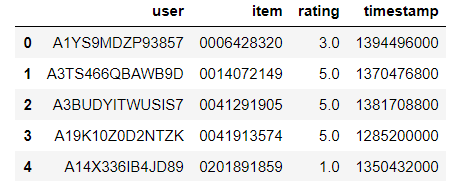
\includegraphics[height=4cm]{figure1.png}
\caption{Samples from Amazon review datasets}
\end{figure}


\end{frame}










\begin{frame}{Datasets}


\begin{figure}
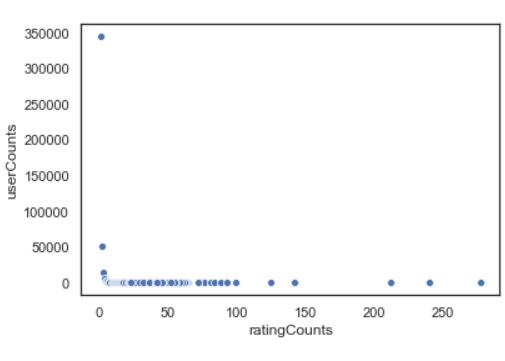
\includegraphics[height=5cm]{figure2.png}
\caption{Statistics of users' ratings}
\end{figure}


\end{frame}










\begin{frame}{Datasets}


\begin{figure}
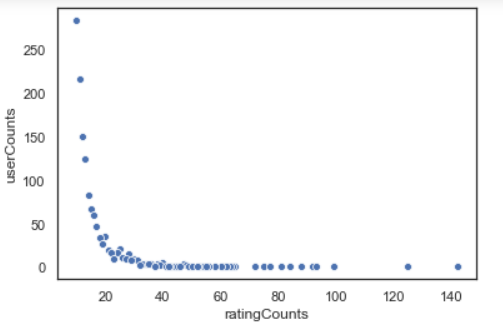
\includegraphics[height=5cm]{figure3.png}
\caption{Statistics of users' ratings}
\end{figure}




\end{frame}









\begin{frame}{Datasets}

\begin{table}[]
    \centering
    \begin{tabular}{cccc}
    \toprule  
    Datasets & Users & Items & Ratings\\
    \midrule  
    Instant Video & 426922 & 23965 & 583933  \\
    Musical Instrument & 339231 & 83046 & 500176  \\
    \bottomrule
    \end{tabular}
    \caption{Statistics of the raw datasets}
\end{table}


\begin{table}[]
    \centering
    \begin{tabular}{cccc}
    \toprule  
    Datasets & Users & Items & Ratings\\
    \midrule  
    Instant Video & 1372 & 7957 & 23181 \\
    Musical Instrument & 2270 & 21464 & 38404 \\
    \bottomrule
    \end{tabular}
    \caption{Statistics of the preprocessed datasets}
\end{table}
    
    
\end{frame}









\begin{frame}{Evaluation}


\begin{table}[htbp]
  \centering
  
    \begin{tabular}{c|ccc|ccc}
    \hline
    Datasets & \multicolumn{3}{c|}{Instant Video} & \multicolumn{3}{c}{Musical Instrument} \\
    \hline
    \hline
    Measures@10(\%) & P     & R     & F1    & P     & R     & F1 \\
    \hline
    SVD   & 0.984 & 2.065 & 1.285 &       &       &  \\
    kNN   & 0.496 & 1.183 & 0.681 &       &       &  \\
    \hline
    \hline
    \end{tabular}%
  \label{tab:addlabel}%
  \caption{The performance of baselines}
\end{table}%

\begin{align*}
&P@N = \frac{1}{M} \sum_u P_u@N = \frac{1}{M} \sum_u \frac{|R_u \cap T_u|}{|R_u|}\\
&R@N = \frac{1}{M} \sum_u R_u@N = \frac{1}{M} \sum_u \frac{|R_u \cap T_u|}{|T_u|}\\
&F_1@N = \frac{1}{M} \sum_u F_{1u}@N = \frac{1}{M} \sum_u \frac{2 \cdot P_u@N \cdot R_u@N }{P_u@N\ +\ R_u@N}
\end{align*} 


\end{frame}











\begin{frame}{Our model}


For the reinforcement learning stage,
\begin{itemize}
    \item \textbf{Observation} The prespecified user $u$ and all users' purchasing history. 
    \item \textbf{Action} Output $K$ neighbors of the user $u$.
    \item \textbf{Policy} $Upper\ Confidence\ Bounds$ methods.
    \begin{align*}
        \bar{x}_{u'}(t) + \sqrt{\frac{2 \ln{t}}{T_{u',t}}}
    \end{align*}
\end{itemize}


\end{frame}










\begin{frame}{Our model}


For the superposed Hawkes process learning,
\begin{itemize}
    \item \textbf{Merge}  Combining the purchasing history of the $K$ neighbors and the prespecified user u.
    \item \textbf{MLE} 
    \begin{align*}
      \min - \log \mathcal{L} (\mathcal{H}_{train}^{super}; \left\{\lambda_c^u \right\}_{c \in C}) 
    \end{align*}
    \item \textbf{Reward} 
    \begin{align*}
        \begin{matrix}
            - \sum_{c \in C} \left(N_c^u(t_{test}) - \int_{t_{test}} \lambda_c^u(s) \, ds \right)^2
        \end{matrix}
    \end{align*}
    
\end{itemize}


\end{frame}



\end{document}
